% options:
% thesis=B bachelor's thesis
% thesis=M master's thesis
% czech thesis in Czech language
% english thesis in English language

\documentclass[thesis=M,english]{FITthesis}[2011/07/15]
\bibliographystyle{iso690}

\usepackage[utf8]{inputenc} % LaTeX source encoded as UTF-8

\usepackage{graphicx} %graphics files inclusion
% \usepackage{subfig} %subfigures
% \usepackage{amsmath} %advanced maths
% \usepackage{amssymb} %additional math symbols

% source code
\usepackage{float}
\usepackage{listings}
\usepackage{color}
\definecolor{gray}{rgb}{0.4,0.4,0.4}
\definecolor{darkblue}{rgb}{0.0,0.0,0.6}
\definecolor{cyan}{rgb}{0.0,0.6,0.6}

\lstset{
  basicstyle=\ttfamily,
  columns=fullflexible,
  showstringspaces=false,
  commentstyle=\color{gray}\upshape
}
\lstdefinelanguage{XML}
{
  basicstyle=\ttfamily\color{darkblue}\bfseries,
  morestring=[b]",
  morestring=[s]{>}{<},
  morecomment=[s]{<?}{?>},
  stringstyle=\color{black},
  identifierstyle=\color{darkblue},
  keywordstyle=\color{cyan},
  morekeywords={link}
}

\lstset{language=XML}

% BibTeX
\usepackage{url}
 
\floatstyle{ruled}
\newfloat{program}{thp}{lop}
\floatname{program}{Code}

% list of acronyms
\usepackage[acronym,nonumberlist,toc,numberedsection=autolabel]{glossaries}
\iflanguage{czech}{\renewcommand*{\acronymname}{Seznam pou{\v z}it{\' y}ch zkratek}}{}
\makeglossaries

% % % % % % % % % % % % % % % % % % % % % % % % % % % % % % % % % % % 
% % % % % % % % % % % % % % % % % % % % % % % % % % % % % % % % % % % 
\department{Department of theoretical computer science}
\title{Admission procedure \\ \hspace*{3.6mm} Automatic processing of applications\\ \hspace*{3.6mm} for master's study
program} 
\newcommand{\rawtitle}{Admission procedure Automatic processing of applications for master's study program}
 
\author{Ján Ondrušek} %author's name without academic degrees
\authorWithDegrees{Bc. Ján Ondrušek} %author's name with academic degrees
\supervisor{Ing. Tomáš Kadlec}
\acknowledgements{I would like to thank my family and friends for support during writing this thesis.}
\abstractCS{Primárnym cieľom tejto diplomovej práce je analyzovať Řád přijímacího řízení ČVUT a Směrnici děkana pro
přijímací řízení na ČVUT Fakultě informačních technologií. Implementovať RESTful API, ktoré vystaví funkcionalitu
backendu pre prijímací proces s použitím Business Process Management stroja.} 
\abstractEN{Primary aim of this thesis is to analyse Conditions for admission and Dean's directive for admission process
to master's study programme at CTU FIT. Implement RESTful API, which exposes backend functionality for admission
processing using Business Process Management.}
\placeForDeclarationOfAuthenticity{Prague}
%where you have signed the declaration
\keywordsCS{Spracovanie prihlášok, RESTful API, BPM, jBPM, Spring, Spring Roo}
\keywordsEN{Admission procedure, RESTful API, BPM, jBPM, Spring, Spring Roo}

\begin{document}

\newacronym{API}{API}{Application Programming Interface}
\newacronym{BPM}{BPM}{Business process management}
\newacronym{BPEL}{BPEL}{Business Process Execution Language}
\newacronym{BPEL4WS}{BPEL4WS}{Business Process Execution Language for Web Services}
\newacronym{BPMI}{BPMI}{Business Process Modeling Initiative}
\newacronym{BPML}{BPML}{Business Process Modeling Language}
\newacronym{BPMN}{BPMN}{Business Process Model and Notation}
\newacronym{BPSS}{BPSS}{Business Process Specification System}
\newacronym{CDI}{CDI}{Contexts and Dependency Inject}
\newacronym{DI}{DI}{Dependency Injection}
\newacronym{EDGE}{EDGE}{Enhanced Data rates for GSM Evolution}
\newacronym{FIS}{FIS}{Faculty Information System}
\newacronym{HATEOAS}{HATEOAS}{Hypermedia As The Engine Of Application State}
\newacronym{HTTP}{HTTP}{Hypertext Transfer Protocol}
\newacronym{ICT}{ICT}{Information and communication technologies}
\newacronym{IT}{IT}{Information Technology}
\newacronym{JAXRS}{JAX-RS}{Java API for RESTful Web Services}
\newacronym{JAXWS}{JAX-WS}{Java API for XML Web Services}
\newacronym{JSON}{JSON}{JavaScript Object Notation}
\newacronym{KOS}{KOS}{KOmponenta Studium, Study Information System at CTU}
\newacronym{MDA}{MDA}{Model-Driven Architecture}
\newacronym{MIME}{MIME}{Multipurpose Internet Mail Extensions}
\newacronym{OMG}{OMG}{Object Management Group}
\newacronym{OSS}{OSS}{Open-source software}
\newacronym{POM}{POM}{Project Object Model}
\newacronym{REST}{REST}{REpresentational State Transfer}
\newacronym{RESTful}{RESTful}{With application of REST principles}
\newacronym{SOA}{SOA}{Service-oriented architecture}
\newacronym{SOAP}{SOAP}{Simple Object Access Protocol}
\newacronym{URI}{URI}{Uniform Resource Identifier}
\newacronym{XML}{XML}{Extensible Markup Language}
\newacronym{W3C}{W3C}{World Wide Web Consortium}
\newacronym{WSCDL}{WS-CDL}{Web Services Choreography Description Language}
\newacronym{WfMC}{WfMC}{Workflow Management Coalition}
\newacronym{WSBPEL}{WSBPEL}{Web Services Business Process Execution Language}

\begin{introduction}
	\section{Motivation and objectives}

	Every year hundreds of high school graduates apply for studies at Czech Technical University, Faculty of informatics.
	This raises certain requirements including managing, storing, analysing and processing of all these applications.
	Each application has its own life cycle, which begins with filling out an on-line form and continues through various
	steps which an applicant has to pass. The life cycle ends when a decision of acceptance is delivered to the applicant
	and he either enrolls in the studies or not.
	
	We live in the world of new era of the Internet. Everything goes on-line, web and the latest trend - everything goes
	mobile. People want things to happen very quickly. They want to access all the information fast, now.
	
	Students and applicants are no different. They expect from this prestigious University, especially from Faculty of
	informatics, most modern and useful gadgets when it comes to software and web.
	
	\section{How do things work now}
	
	Currently all applications are processed rather manually. Many man days of administrative work are consumed during the
	process. Although an electronic form is filled in and submitted by an applicant, the rest of actions almost exclusively
	fall into the hands of Study Department staff. Some of the work is handled by simple scripts or other utilities. The
	question is: Why don't we do most of the work automatically?
	
	This work is monotonous and can even lead to men's frustration.
	
	\section{What should be achieved}
	
	Courses at Faculty of informatics teach its students to handle various programming languages, web technologies and
	techniques.
	We all know what to expect from a working web application and good looking one is a bonus. This is why knowledge of
	faculty's students should be used for good of their successors. Fast, reliable, informative and functional system will
	make them fell more comfortable and perhaps could even some precious time.
	
	Ideal state would be to accept on-line application and automatically generate invitations for applicants, that should
	attend a test. After the test, process all results and generate decision of acceptance letter for all who passed the
	test or are accepted without it. The only manual interventions that will remain is to accept apology, appeal and insert
	the letters into the envelopes.
	
	\section{Let's make things better}
	
	Taking the above written into account, this might be a good idea for a master's or bachelor's thesis. However if we
	want to use all available technologies that have become popular in past years and to automatize majority of admission
	processing, it turns out to be a very complex project. So why not to create several teams and split necessary work into
	multiple, both bachelor's and master's, thesis?
	
	This is how project Přiříz was born. It includes web interface for both students and Study Department staff, native
	Android application and RESTful API with BPM processing machine, which is a subject of my master's thesis.
	 
\end{introduction}
\chapter{RESTful API with JAX-RS}\label{rest}

	Nowadays, Internet consumers demand fast growth of various services and integration of their favourite ones. As en
	example I can point out synchronization of contact list between very popular social networks, e-mail providers and
	phone contact lists. 
	
	Other example may be growing amount of \verb|mashups|\footnote{Applications that are created via
	combination of multiple different services. Such application, almost exclusively web based, can be created very quickly
	by consuming several \gls{API}s. Not necessarily from the same provider.} and uncountable number of
	\verb|startups|\footnote{Constantly rising amount of web applications that focus on fast growth of attracted users.
	They offer various services, which are often very innovative and experimental. One successful example is popular
	social network and my favorite information channel - Twitter.}, who often provide RESTful or different type of public
	\gls{API}.

	\section{Talking about REST, what is it?}
	
	\gls{REST} or RESTful programming is not defined by any official standard and there are no official guidelines or rules
	for it.
	So what is it then? It is and architectural and programming style for Web, where a set of constraints is defined. Lots
	of text has been written about it during past years and describing the whole idea of REST is out of scope of this
	master's thesis. I can however try to point out the most significant, important and basically, what I personally
	managed to adopt.
	
	\subsection{Main principles of REST, RESTful web service}
	
	There are several architectural principles that one should keep in mind when thinking of REST \cite[p.~3]{restful}:
	
	\begin{itemize}
	  	\item \textbf{Addressable resources} 
	  	The key abstraction of information and data in REST is a resource, and each resource must be addressable via a
	  	\gls{URI}.
		\item \textbf{A uniform, constrained interface}
		Use a small set of well-defined methods to manipulate your resources.
		\item \textbf{Representation-oriented}
		You interact with services using representations of that service. A resource referenced by one URI can have different
		formats. Different platforms need different formats. For example, browsers need HTML, JavaScript needs JSON (JavaScript
		Object Notation), and a Java application may need XML.
		\item \textbf{Communicate statelessly}
		Stateless applications are easier to scale.
		\item \textbf{\gls{HATEOAS}}
		Let your data formats drive state transitions in your applications.
	\end{itemize}
	
	\gls{HATEOAS} is often understood as a core principle of \gls{REST}. It carries an idea of resource representation via
	links and stateless implementation of services.
	
	RESTful web services are the result of applying these constraints to services that utilize web standards such as
	\gls{URI}s, \gls{HTTP}, \gls{XML}, and \gls{JSON}.
	
	\subsection{Back to the roots, HTTP is reborn}
	
	\gls{SOA} has been in this world for a long time. Many different approaches and technologies exist to implement it.
	From those worth to mention: DCE, CORBA, Java RMI, \ldots They offer robust standards, one can build large, complex
	and scalable systems on top of it, but there is a cost. They often bring huge complexity and maintenance requirements
	into place.
	
	Currently, when one says \gls{SOA}, it often evokes \gls{SOAP} in a mind that spent several years using technologies
	mentioned above. This however is not a bad thing. \gls{SOAP} is used very widely and is perfectly suitable for
	developing services and \gls{API}s. But it is definitely not a lightweight technology and it is not ideal for
	everything. Its most common use case is for server-server communication in enterprise systems.
	
	Nowadays, we need something quickly adoptable, widely spreadable, platform and technology independent and client
	oriented. This needs a completely different approach and new way of thinking when it comes to \gls{SOA}. It is about
	Web, so why not to start with something that is Web, as we see it today, based on? Yes, it is \gls{HTTP}.
	
	Although \gls{REST} is not protocol specific, when saying \gls{REST} it usually automatically means \gls{REST} +
	\gls{HTTP}. No wonder. \gls{HTTP} is perfectly suitable for client-server \gls{SOA}, it is just about the way of
	thinking. It offers transport layer, request-response mechanism, descriptive responses, caching mechanism and many
	more. It is true that in past years, when various types of web applications started to appear, many web developers
	limited their thinking and use of \gls{HTTP} to two basic cases:
	
	\begin{itemize}
	  \item GET a page with \gls{URI}, perhaps containing a few query parameters
	  \item POST a form
	\end{itemize}
	
	\begin{program}
	\caption{HTTP GET request/response example of a standard web page}\label{http_get_web}
	\begin{verbatim}
	GET /index.html HTTP/1.1
	User-Agent: curl/7.24.0 (i686-pc-cygwin) ...
	Host: www.google.sk
	Accept: text/html,application/xhtml+xml,application/xml;q=0.9,*/*;q=0.8
	Accept-Language: sk-sk,en;q=0.5

	HTTP/1.1 200 OK
	Date: Thu, 07 Jun 2012 11:25:15 GMT
	Expires: -1
	Cache-Control: private, max-age=0
	Content-Type: text/html; charset=ISO-8859-2
	Set-Cookie: ... expires= ...; path=/; domain=.google.sk
	Set-Cookie: ... expires= ...; path=/; domain=.google.sk; HttpOnly
	Server: gws
	X-XSS-Protection: 1; mode=block
	X-Frame-Options: SAMEORIGIN
	Transfer-Encoding: chunked

	<!doctype html><html ...><head> ... <body> ...
	\end{verbatim}
	\end{program}
	
	The example above \ref{http_get_web} shows most common HTTP request and response, when browsing the web via standard
	web browser. It requests object \textbf{/index.html} using \textbf{GET} method placed on host \textbf{www.google.sk}.
	My client also put several HTTP headers into the request:
	
	\begin{itemize}
	  \item \textbf{Accept:} text/html,application/xhtml+xml,application/xml;q=0.9,*/*;q=0.8
	  \item \textbf{Accept-Language:} sk-sk,en;q=0.5
	\end{itemize}
	
	Also the request does not contain any request body, as it is GETting information from the server. 
	
	The response of the message received is 200, which means OK - success. An overview of all available HTTP response codes
	can be found on-line at \cite{httpcodes}. \textbf{Content-type} header of the response message says that the body
	received is of type HTML.
	
	RESTful web service needs more than that and luckily \gls{HTTP} offers much more. It will be better to point out its
	features in a relationship to each of REST's architectural principles.
	
	\subsection{Addressable resources, URIs and links}
	
	Each \textbf{resource} in a system should be reachable through a \textbf{unique identifier}. When reflected to the idea
	of REST and HTTP, URIs will automatically come to mind. The format of a URI looks like this \cite{uri}:
	
	\begin{verbatim}
	<scheme>://<authority><path>?<query>
	\end{verbatim}
	
	The above is a citation directly from RFC, but for purposes of this master's thesis should be rewritten into more
	detailed form:
	
	\begin{verbatim}
	<scheme>://<host>:<port>/<path>?<queryString>#<fragment>
	\end{verbatim}
	
	Where in the RESTful world these parts usually mean:
	\begin{itemize}
	  \item \textbf{scheme} typically \textbf{http} or \textbf{https}
	  \item \textbf{host} aka server name, e.g. \textbf{fit.cvut.cz} and \textbf{port}
	  \item \textbf{path} to the resource on server, e.g. \textbf{/admission/123-456-01}
	  \item \textbf{queryString} after the \textbf{?} is typically used for a set of resources and can be a page number,
	  number of items in the set, or a filter definition and many more, e.g. \textbf{?page=1\&limit=10}
	  \item \textbf{fragment} after the \textbf{\#} usually points to a certain place in a document
	\end{itemize}
	
	An example of such URI pointing to a set of resources may be:
	
	\begin{verbatim}
	http://pririz.is.fit.cvut.cz:9090/admission/services/admission
		?page=2&count=20
	\end{verbatim}
	 
	An example of URI pointing to a concrete single resource:
	
	\begin{verbatim}
	http://pririz.is.fit.cvut.cz:9090/admission/services/admission
	/123-456-01
	\end{verbatim}
	
	Characters allowed in \gls{URI} string are all alphanumeric, comma, dash, asterisk and underscore. Space is converted
	into plus and other characters are encoded using specific schema into a two digit hexadecimal number, which is appended
	to the \% character.
	
	\subsection{The uniform, constrained interface, HTTP methods}
	
	This is probably the prettiest part of a relationship between REST and HTTP. It may be a bit difficult to adopt this
	principle for a person, who spent a couple of years developing CORBA or SOAP services.  There is a finite set of HTTP
	methods and all REST operations have to stick to it. All other parameters describing operations must be omitted from
	\gls{URI}.

	Let's see what \gls{HTTP} offers:
	
	\begin{table}[h]\centering
	 	\begin{minipage}{12.9cm}
		\begin{tabular}{l|c|c|p{6cm}}
		\hline
		Method & \verb|Idempotent|\footnote{Idempotent means that no matter how many times you apply the operation, 
		the result is always the same.} & \verb|Safe|\footnote{Safe means that invoking an operation does not change the 
		state of the server at all. This means that, other than request load, the operation will not affect the server.} 
		& Operation(s)\\
		\hline
		GET & yes & yes & read - query information from a server\\
		POST & no & no & write, update - both can change a server state in a unique way each time executed\\
		PUT & yes & no & update for the known resource, updating the same resource more than once does not effect it\\
		DELETE & yes & no & delete - removes resource\\
		HEAD & yes & yes & read without response body, returns only response headers\\
		OPTIONS & yes & yes & information about communication options with server\\
		\end{tabular}
	    \renewcommand{\footnoterule}{}
	    \end{minipage}
	\caption{An overview of HTTP methods and their roles in a RESTful service}
	\label{http_methods}
	\end{table}
	
	HTTP contains a few other methods (TRACE, CONNECT), which are unimportant for purposes of RESTful services.
	
	What is more interesting, nowadays a couple of non-HTTP methods have appeared, which may be good for RESTful service
	design in the future. Namely PATCH (very similar to the PATCH method found in \verb|WebDAV|\footnote{WebDAV stands for
	Web-based Distributed Authoring and Versioning. It is a set of extensions to the HTTP protocol which allows users to 
	collaboratively edit and manage files on remote web servers.}) and MERGE. According to various sources I have found on
	the web, namely \cite{httppatch}, \cite{msdnpatchmerge} or \cite{rfc2616}, they may appear in further HTTP
	specifications. They are not a part of current HTTP 1.1.
	
	PATCH and MERGE are used for partial update of known resources that contain large amount od data and updating the whole
	object would be a lengthy and ineffective operation. This however can be simulated using POST and specifying detailed
	path of the resource via URI.
	
	\subsection{Representation-oriented}
	
	I already described that each resource has its own URI and client-server principle using HTTP. Its methods allow the
	client to receive current representation via GET method, remove it from server via DELETE or change the representation
	via POST and PUT methods. Concrete representation can be received in JSON, XML, YAML or any other format one can
	imagine.
	
	Representation format is agreed between client and server in a RESTful system interaction. HTTP offers such feature
	by specifying \textbf{Content-Type} header. Its value string is represented by \gls{MIME} format:
	
	\begin{verbatim}
	<type>/<subtype>[;name=value;name=value...]
	\end{verbatim}
	
	An example may be:
	
	\begin{verbatim}
	text/html; charset=utf-8
	text/xml
	text/json
	application/xml
	application/json
	\end{verbatim}
	
	To choose preferred format(s), client can specify \textbf{Accept} HTTP header in a request. Now it becomes more clear
	how REST and HTTP perfectly fit each other. Together they offer addresability, method choice and object representation
	format.
	
	\subsection{Communicate statelessly, (no)sessions}
	
	HTTP offers powerful client session management, which is commonly used when browsing the web via traditional web
	browser. It stores so called \textbf{Cookies} when a server asks for it in response headers, which are then sent back
	to the server with subsequent requests. This is how the server handles stateful interaction with the client over HTTP.
	
	Stateless communication in REST means that there is no client session data stored on a server. In other words, none of
	the above is performed. It does not mean that RESTful application cannot be stateful, though.
	
	Reason for this is simplicity, which further leads to easily scalable RESTful service. It is generally much less
	difficult to build a cluster of stateless applications than to handle session replication and possibly another service
	layer.
	
	\subsection{HATEOAS}
	
	\cite[p.~11]{restful} Hypermedia is a document-centric approach with the added support for embedding links to other
	services and information within that document format.
	
	There are several ways how to understand any apply this RESTful architectural principle. One use case is to add
	hyperlinks when composing complex and large objects. This avoids unexpected server load, delay in response to the
	client and helps to reference dependent or embedded objects without bloating the response.
	
	An example of server response without any hyperlinks:
	
	\begin{lstlisting}[tabsize=2]
	<terms>
		<term>
			...
			<registrations>
				<registration>
					<admission>
						<code>96858805</code>
						<type>P</type>
						<accepted>false</accepted>
						... some huge object containing 
						a lot of information
					</admission>
					<term>
						<dateOfTerm>2012-05-10...</dateOfTerm>
						<room>BS</room>
						<capacity>1500</capacity>
						<registerFrom>2012-05-03...</registerFrom>
						<registerTo>2012-05-08...</registerTo>
						<apologyTo>2012-05-08...</apologyTo>
						... another huge object containing 
						a lot of information, graph can be even circular
					</term>
				</registration>
				...
			</registrations>
			...
		</term>
		...
	</terms>
	\end{lstlisting}
	
	Let's apply embedded hyperlinks on the document above:
	
	\begin{lstlisting}[tabsize=2]
	<terms>
		<term>
			...
			<registrations>
				<registration>
					<admission>
						<link href="http://.../admission/96858805" 
						method="GET" rel="admission" />
					</admission>
					<term>
						<link href="http://.../term
						/dateOfTerm:2012-05-10T14:22:00/room:BS"
							method="GET" rel="term" />
					</term>
				</registration>
				...
			</registrations>
			...
		</term>
		...
	</terms>
	\end{lstlisting}
	
	This concept of HATEOAS is called aggregation. But it isn't everything. In a case that the server would return
	thousands of term objects and each of them would contain thousands of registrations including admissions, the response
	would be, again, very large. However, there is one even more interesting part of HATEOAS - the \uv{engine}.
	
	Core of the engine principle is not to return the whole set of object available, but just a subset of it and to
	tell the client, where to find the rest:
	
	\begin{lstlisting}[tabsize=2]
	<terms>
		<count>5</count>
		<totalCount>123</totalCount>
		<link href="http://.../term?page=3&count=5" method="GET" 
			rel="next" />
		<link href="http://.../term?page=1&count=5" method="GET" 
			rel="previous" />
		<term>
			...
			<registrations>
				<registration>
					<admission>
						<accepted>false</accepted>
						<link href="http://.../admission/96858805" 
							method="GET" rel="admission" />
					</admission>
					<term>
						<link href="http://.../term
						/dateOfTerm:2012-05-10T14:22:00/room:BS"
							method="GET" rel="term" />
					</term>
				</registration>
				...
			</registrations>
			...
		</term>
		...
	</terms>
	\end{lstlisting}
	
	This approach saves a lot of server resources and prevents client from unexpected delays due to large responses. Such
	response should be always returned in constant time, because the request query defines its maximum size - number of
	objects.
	
	\section{REST, Java and JAX-RS}

\chapter{Přiříz architecture and requirements}\label{architecture}

	Previous chapters should provide enough information to understand basic principles of a RESTful service and benefits of
	using BPM. Discussion about the two mentioned will become more concrete from now on, because admission process will be
	taken into account.
	
	As a result of this master's thesis a working application is implemented. Further referred as \textbf{RESTful API} and
	it integrates both technologies.
	 	
	This chapter describes requirements for application functionality and its role in the architecture of the whole project
	currently running at CTU FIT.

	\section{\gls{FIS}}
	
	The project covers activities related to information system development CTU. It is quite complicated and long term
	project involving more than dozen people in various roles. RESTful API with two other applications directly
	interconnected is just a part of it and together they form \textbf{Přiříz} component \ref{fig:fis_architecture}.
	
	\newpage
	\begin{figure}[h]
		\label{fig:fis_architecture}
	  	\centering
	    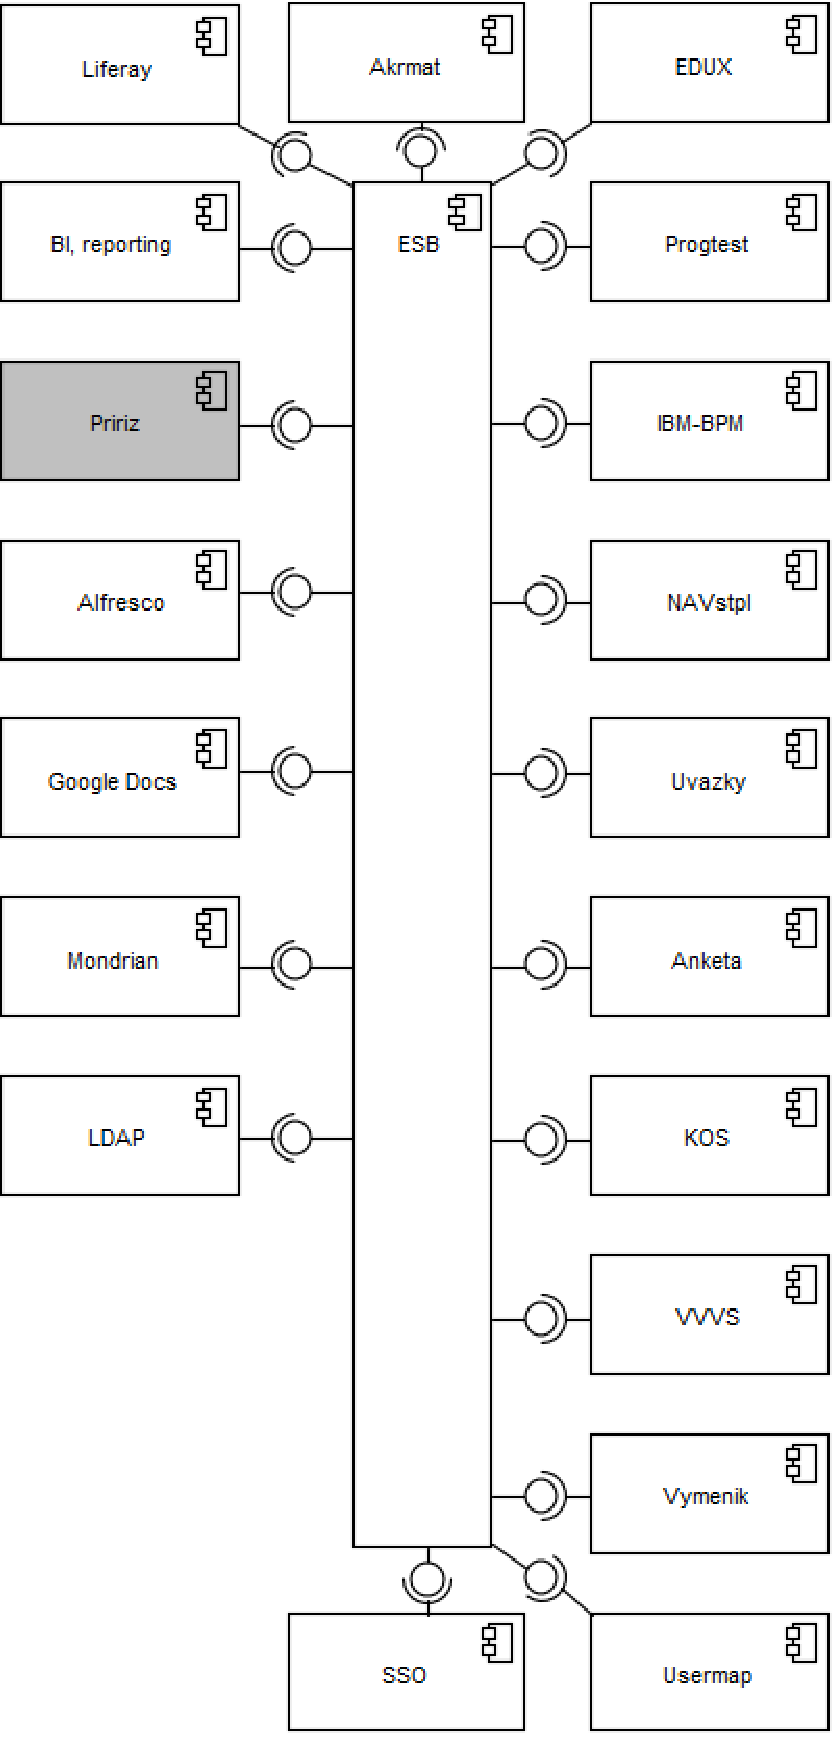
\includegraphics[width=6cm]{figures/fis_architecture}
	  	\caption{FIS architecture}
	\end{figure}
	
	\section{Catalogue of requirements}
	
	This section lists requirements for the RESTful API. 
	
	\subsection{Functional requirements}
	
	Functional requirements define which services should system provide. 
	\begin{itemize}
		\item F00 Admission import
	
		data import from e-admission, on-line CTU form
		
		\item F01 Admission evidence
	
		evidence of valid admissions
		
		\item F01.1 Admission detail
		
		detailed information about admission and admissioner
		
		\item F01.2 Admission edit
		
		update of allowed admission data
		
		\item F01.3 Password reset
		
		allow password reset/recovery to a valid user account related to the admission
	
		\item F02 Term evidence
	
		entrance exam term evidence
		
		\item F02.1 Term management
		
		entrance exam term management
		
		\item F02.2 Enrollment term management
	
		enrollment term of accepted admissioners management
		
		\item F02.3 Term registrations evidence
	
		Entrance exam or enrollment term registrations of admissionsers evidence
	
		\item F03 Statistics
	
		various statistics of this year's admission process
	
		\item F04 User management
	
		password change
	
		\item F05 Admission state
	
		view current state of admission
		
		\item F05.1 Entrance exam registration
		
		allow an admissioner to book entrance exam term
		
		\item F05.2 Entrance exam apology
		
		allow an admissioner to apologise from the entrance exam registration
		
		\item F05.3 Enrollment registration
		
		allow an admissioner to book enrollment term
		
		\item F05.4 Enrollment apology
		
		allow an admissioner to apologise from the enrollment registration
		
		\item F06 Admission process management
		
		allow management of an admission during admission process
		
		\item F06.1 Send e-mails
		
		allow sending of informative e-mail
		
		\item F06.2 User action processing
		
		allow processing of user actions during admission process
		
		\item F07 File number administration
		
		allow file number assignment to documents communicated with an admissioner
		
		\item F08 Document creation
		
		allow document creation of various types for an admissioner 
	\end{itemize}
	
	\subsection{Non-functional requirements}
	
	Non-functional requirements do not directly define system functionality, but describe constraints or general
	properties.
	
	\begin{itemize}
		\item NF01 User action processing
	
		jBPM engine requires local TaskService server to handle user actions in process
		
		\item NF02 E-mail server configuration

		jBPM engine requires properly configured mail sender to be able to use CTU's mail server
		
		\item NF03 Technologies
		\label{NF03}
		
		use the following for implementation: JEE, Apache Maven, jBPM, Spring Framework, Spring Roo, JPA
		
		\item NF04 System and web service security
		
		system and web services will be secured
		
		\item NF04.1 User roles and permissions
		
		security will be handled by user roles and permissions
		
		\item NF05 MySQL database
		
		primary DBMS will be MySQL
		
		\item NF06 Server Tomcat
		
		RESTful API will be able run on Apache Tomcat servlet container
		
		\item NF07 Performance under load
		
		system must handle 250 concurrent users and 2500 total users
		
		\item NF07.1 Scaling
		
		system must be able to split load among multiple instances
	\end{itemize}
	
	During the development process several changes were made to the catalogue of requirements. RESTful API team and UI team
	switched responsibilities for  F07, F08. F03 was descoped but can be implemented with relatively small effort when
	needed.
	
	NF07.1 is a matter of infrastructure. While this work was being created, only one virtual server was available for the
	whole Přiříz project and makes no sense to configure multiple instances on a single machine.
	
	\section{Who and how will use RESTful API?}\label{sec:who_will_use}
	
	I already mentioned that RESTful API will be consumed by two different teams \ref{fig:pririz_project_component}. This
	is their simplified requirements catalogue - functional requirements only:
	
	\begin{figure}[h]
	  	\centering
	  	\label{fig:pririz_project_component}
	    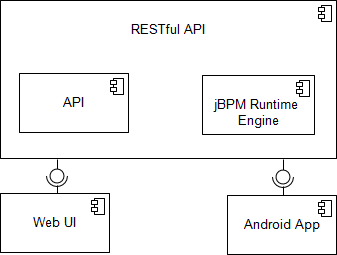
\includegraphics[width=8cm]{figures/pririz_project_component}
	  	\caption{Přiříz project components}
	\end{figure} 
	
	\begin{itemize}
		\item Android team

		Responsible for native Android application development. Its tasks are:
			\begin{itemize}
				\item allow to log-in in various user roles
				\item log-out
				\item barcode identification
				\item view admission/admissioner information
				\item save admission result - entrance exam score
				\item take a picture of a document and upload it to server 
			\end{itemize}
	  \item UI team
	  
	  	Implements web interface. This allows admissioners and CTU FIT's employees to interact with admissions and
	  	manage them during admission process.
		\begin{itemize}
			\item Admission/Admissioner
			\begin{itemize}
				\item log-in/log-out
				\item view personal information
				\item book a term (entrance exam, enrollment)
				\item apologise from a term registration
				\item change/reset password
			\end{itemize}
			\item Employee (Study Department staff, sub dean, Faculty departments staff)
			\begin{itemize}
			  	\item log-in/log-out
				\item list admissions, filter
				\item view admission detail
				\item edit/delete admission
				\item reset user's password by admission
				\item view terms (entrance exam, enrollment)
				\item create/edit/delete terms
				\item import admission data from \gls{KOS}
				\item view study programs
				\item edit/delete study programme
				\item confirm admissioner's attendance at entrance exam or enrollment
				\item accept or decline admissioner's apology
				\item edit properties of an admission process 
				\item view statistics
				\item change password
			\end{itemize}
		\end{itemize} 
	\end{itemize}

	Although UI team has quite a long list of task when compared to Android's, they practically overlap.
	This is why both (and for future all) teams are going to share the same API and RESTful API will handle all consumers
	the same way.

	All requirements from the list above, but those platform specific, will use RESTful API as a backend and should not
	store any persistent data on their own. Platform specific means that they must store runtime data on their own. An
	example may be HTTP session or other temporaries.

	The task for RESTful API team is to expose a public API, which will satisfy requirements from the list above.
	 
\chapter{Chosen technologies}\label{cha:technologies}

	This chapter describes pros and cons of available tools, frameworks and architectural patterns, that may be used and
	explains why and which technologies I finally selected.
	
	One of the non-functional requirements from the previous chapter \ref{itm:NF03} talks about technologies, which should
	be used. The truth is that NF03 was back-added after discussion described in this chapter.

	\section{REST vs. SOAP}
	
	Although implementing a RESTful API is one of the main topics of this master's thesis, it is good to compare other
	possibilities too. Currently the most commonly used technology to build SOA in addition to REST is SOAP. So what are
	the differences between them? Why should I not use SOAP, when thousands of enterprise systems are using it?
	
	Sometimes people talk about SOAP like it was something that is deprecated, or even dead and REST is its successor and
	is much better and modern. This is not true and not even part of it. REST is no revolution in SOA, but rather
	an evolution. SOAP has its place when it comes to a question of implementing services or APIs and so does REST. The
	main difference is: \textbf{SOAP} is aimed for \textbf{server-server} communication and \textbf{REST} is more suitable
	for \textbf{client-server} communication.
	
	Let's forget about the RESTful API requirement and make it just an API. What are the pros and cons of REST, resp. SOAP
	if I could choose one or the another on my own? The only things that I have to keep in mind: I'm implementing an API
	for admission processing and I have two different API consumers using two various platforms \ref{sec:who_will_use}.
	
	\begin{table}[h]\centering
	 	\begin{minipage}{12.9cm}
		\begin{tabular}{p{2cm}|p{4.75cm}|p{4.75cm}}
		\hline
		& REST & SOAP\\
		\hline
		Data Format & XML, JSON, YAML, \ldots & XML \\
		Transport & agnostic, but very tightly coupled with HTTP, unlikely to use anything else & agnostic \\
		Error handling & implementation specific & built in \\
		Primary use & client-server directly & server-server, possibly via mediators \\
		\verb|CRUD|\footnote{Create Read Update Delete} & HTTP methods & implementation specific \\
		Interface description & text description, XSD for XML representation & standardized WSDL, optional XSD \\
		Tools availability & lacking, partial & outstanding \\
		Security & HTTPS, implementation specific  & built in, WS-Security \\
		\hline
		Pros & Lightweight & Standards \\
			 & Space saving formats & Extensible \\
			 & Easy to learn & Tool support \\
			 &  & Type checking \\
			 &  & Rigid \\
		Cons & HTTP dependency & Bloating data format \\
			 & Lacking standards & Complexity and learning curve \\
			 & Lacking tools &  \\
			 & Assumes point-to-point use &  \\
		\end{tabular}
	    \renewcommand{\footnoterule}{}
	    \end{minipage}
	\caption{REST vs. SOAP properties}
	\label{tab:rest_vs_soap}
	\end{table}
	
	Does not look very good for REST from the overview above. Using simple math, it has less pros and more cons. But does
	it mean that SOAP should be chosen for API that Přiříz project needs?
	
	Android team uses a mobile phone device, which is definitely a client. What about the Web interface? I am not sure
	about the implementation, but from my point of view, it should be a thin client, which stores only necessary runtime
	data for its own needs. No need to synchronize any other data, just consume and present. This means \textbf{two
	clients} will be using the API.
	
	Web interface will be deployed on its own application server somewhere inside the CTU's infrastructure and will use
	fast network connection. On the other hand, Android device will be able to use some wireless fast network - best case.
	But what if the mobile application will be forced to rely on a slower carrier network? EDGE - worst case. The API
	should then try to save as much traffic as it can. XML full of namespaces that \textbf{SOAP} happily uses is
	\textbf{not} the \textbf{right} way, though.
	
	HTTP dependency is not a problem, I would use SOAP over HTTP anyway. Lack of standards is a matter of good design. This
	is why I have to be very careful when exposing new functions or data models. It does not mean that this issue would not
	effect SOAP design.
	
	Lack of tools is a thing that bothers me a bit. If I agree on standardized approach with other teams and we involve a
	bit of communication, hopefully we can get over this one.
	
	So far for the cons of REST. Which pros of SOAP will I miss, if I decided to use REST? Just the tool support.
	
	To sum up, RESTful API would win and therefore I am happy with the original requirement.
	
	\section{BPEL vs. BPMN}
	
	When I started to collect information about BPM and its standards, I found many discussions about older BPEL vs.
	relatively new BPMN, currently available in BPMN 2.0 specification.
	
	\cite{bpm} says that the only standard worth considering is BPEL. This information is a few years old and by the time a
	another player has shown up. BPMN 2.0 became a solid competitor to BPEL.
	
	\cite{oracle_architecture_standards}
	BPEL and BPMN are both \uv{languages} or \uv{notations} for describing and executing business processes. Both are open
	standards. Most business process engines will support one or the other of these languages.
	
	It turns out that BPEL is really well suited to modeling some kinds of processes and BPMN is really well suited to
	modeling other kinds of processes. Of course there is a pretty significant overlap where either will do a great job.
	
	\cite{ms_bpmn_bpel}
	BPMN 2.0 is now a business model that can be executed after implementation details are added. BPMN favors the business
	user, even though a developer can \uv{refine with execution semantics} to make it executable. It is graph based, and
	incorporates user swim lanes, which makes it effective for modelling end to end business processes. 
	
	BPMN 2.0 introduces a standardized file format (previously is was proprietary or converted to XPDL). BPMN looks like a
	version of BPEL where the assigns are tucked away into other activities to clean up the diagram.

	BPEL's nature is still service orchestration, and will be great for building composite services and
	integrating with applications. BPEL will still probably be the choice for developers, where BPMN will be good for the
	pure decision layer and \textbf{Human Task interaction}.
	
	\cite[p.~1]{bpmn}
	The primary goal of BPMN is to provide a notation that is readily understandable by all business users, from the
	business analysts that create the initial drafts of the processes, to the technical developers responsible for
	implementing the technology that will perform those processes, and finally, to the business people who will manage and
	monitor those processes. Thus, BPMN creates a standardized bridge for the gap between the business process design and
	process implementation.
	Another goal  is to ensure that XML languages designed for the execution of \textbf{business processes}, such as
	\gls{WSBPEL}, \textbf{can be visualized} with a business-oriented notation.
	
	Human Task interaction is exactly what admission processing is looking for and visualization of the process is a must.
	It is expected that further modifications of business process model will be performed by non-developers. Therefore an
	user friendly visual modelling tool is required. That is why BPMN 2.0 looks like a good choice. Luckily jBPM, which was
	chosen as a primary technology for this master's thesis, fully implements BPMN 2.0 standard.
	
	\section{Dependency management}
	
	One of the myths about Java development that is well established among people talks about some kind of JAR hell.
	Basically it is a nickname for class loading problem, which used to be an issue some time ago. Nowadays there are tons
	of tools available that effectively solve such issues, one just needs to keep following the progress.
	
	A solution is to use standardized Java project structure, right build tools and dependency management tools. There are
	dozens of such utilities but the two mainstream ones are:
	
	\begin{itemize}
		\item Apache Ant + Apache Ivy

		\cite{ant}		
		Apache Ant is a Java library and command-line tool whose mission is to drive processes described in build files as
		targets and extension points dependent upon each other. The main known usage of Ant is the build of Java applications.
		Ant supplies a number of built-in tasks allowing to compile, assemble, test and run Java applications.
		
		Ant is extremely flexible and does not impose coding conventions or directory layouts to the Java projects which adopt
		it as a build tool.

		Software development projects looking for a solution combining build tool and dependency management can use Ant in
		combination with Apache Ivy.
		
		\cite{ivy}
		Apache Ivy is a dependency manager oriented toward Java dependency management, although it can be used to manage
		dependencies of any kind. Apache Ivy is integrated with Apache Ant, the most popular Java build management system, so
		Apache Ivy follows Apache Ant design principles.
		\item Apache Maven
	  
		\cite{maven}
	  	Apache Maven is a software project management and comprehension tool. Based on the concept of a \gls{POM}, Maven can
	  	manage a project's build, reporting and documentation from a central piece of information.
	  
	  	Maven's primary goal is to allow a developer to comprehend the complete state of a development effort in the
	  	shortest period of time. In order to attain this goal there are several areas of concern that Maven attempts to deal
	  	with:
		
		\begin{itemize}
			\item Making the build process easy
			\item Providing a uniform build system
			\item Providing quality project information
			\item Providing guidelines for best practices development
			\item Allowing transparent migration to new features
		\end{itemize}
	\end{itemize}
	
	Combination of Ant and Ivy is suitable for older, already existing Java projects that use Ant scripts for build
	process. Ivy will allow to remove hard copied JAR files and enable dependency management using remote JAR repositories.
	
	Maven 2 on the other hand is currently the most commonly used project management and comprehension tool. Dependency
	management and project build are just a small part of its capabilities. It offers easy plugin support, from which
	direct deployment to an application server, code coverage and code quality reports might be interesting for this
	project.
	
	Another very nice effect of using is that it leads developers to use standardized project structure. I decided to use
	Maven for RESTful API implementation.
	
	\section{JAX-RS implementation}
	
	In theoretical part \ref{sec:jaxrs} of this work I briefly described JAX-RS. Standard JVM contains only the JAX-RS
	API, but there is no implementation out of box. Luckily, Java developers community is one of the biggest among
	available enterprise solutions and probably the biggest \gls{OSS} enterprise community.
	One of the advantages of such a number of developers is that there is an endless choice of frameworks, utilities and
	other libraries. When it comes to popular JAX-RS implementations these are worth noticing:
	
	\begin{itemize}
	  \item Apache CXF
	  
	  Very complex, popular and pleasant to use.
	  \item Jersey
	  
	  Oracle's reference implementation.
	  \item RESTeasy
	  
	  From JBoss Community.
	\end{itemize}
	
	Personally I tried Apache CXF and RESTeasy. Although any of the above would work well for RESTful API, I have best
	experience with Apache CXF. It offers much more than just plain JAX-RS implementation. Spring framework integration is
	available, error handling is very neat and makes RESTful API server or client development a breeze.
	
	Moreover, it also contains \gls{JAXWS} implementation, which might be useful for future, when SOAP integration is
	required. This will keep REST and SOAP parts consistent across the whole source code.
	
	\section{Spring Core, MVC, Security, \ldots}
	
	When creating a new Java project from scratch, it is good to take a while and think about frameworks, tools and
	possibly other utilities that might simplify development process.
	
	I know I wanted something widely spread because of quick community support and fair documentation state. Utilities like
	Apache Commons, Collection Utils, \ldots is a must. But which framework to choose if there are so many? Well from all
	the available, I am going to look at the most popular ones. Good place to look or ask is Stack Overflow and this is
	what community recommends:
	
	\begin{itemize}
		\item Struts 2
		\item Apache Wicket
		\item Play
		\item Spring 3
		\item pure JEE
	\end{itemize}
	
	The list is surprisingly short. Let's list my requirements too, because this should help me to apply method of
	exclusion:
	
	\begin{itemize}
		\item fully \gls{OSS}
		\item easily configurable
		\item extensible and plugin friendly
		
		No framework contains all one ever needs, therefore it must be easily extensible with custom components.
		\item suitable for integration with other frameworks
		
		I need to integrate JAX-RS with the rest.
		\item large community
		\item good documentation
		\item REST friendly
		
		RESTful application is considered to be a web application, but with one significant difference. When MVC patterrn is
		applied, we can actually skip the View part, because RESTful API generates output based on client-server agreement
		(the Accept HTTP header) and does not need any templates (JSP, FM, Velocity, \ldots). Therefore all JSF based frameworks
		do not fit well, as JAX-RS handles the response and rendering.
	\end{itemize}
	
	After the first round Struts 2 and Apache Wicket have to go. Struts is not complex enough and I did not find any
	examples of integrating JAX-RS with Struts. Although there is a REST plugin for Struts, it is not JAX-RS implementation.
	
	Apache Wicket might be suitable for creating rich web applications, but again, no example of JAX-RS integration with
	itself. I found a few tutorials for RESTful application with Wicket, unfortunately this is not what I was looking for.
	
	Play 2 framework seems very interesting. It is becoming quite popular and has an emerging community. I also
	found a couple of discussions about integrating it with JAX-RS, but they were linking to already non-existing sources
	and so I started to be rather pessimistic about using it for RESTful API. I would definitely give it a try when
	creating a traditional web application.
	
	\section{Spring 3 vs. JEE 6}
	
	I decided to leave a duel of Spring 3 and pure JEE 6 framework at the end. Nowadays one can find dozens of discussions
	about why JEE 6 is better than Spring 3 and why one group of developers claim that they are going to use purely JEE and
	the other wants to stick with Spring 3.
	
	Both specifications came out in about the same time, late 2009. Both will do practically the same for an enterprise
	application, but their philosophy is quite different. While JEE 6 wraps and defines several standards, technologies and
	APIs e.g. Servlet 3.0, EJB 3.1, JAX-RS, JAX-WS, JAXB, JSF, \ldots  - their list is quite long \cite{oracle_jee}. It is
	application server's task to implement JEE 6 standard. Because JEE 6 is not simple, certified application servers
	tend to be quite big. Such application servers are JBoss AS 7, Glassfish 3.1, \ldots
	
	On the other hand there is Spring 3.0. It aims to promote modularity, extensibility and portability across Java EE
	servlet containers - Tomcat, Jetty and others. One can integrate almost everything from the JEE standard with Spring
	and lightweight servlet container, because Spring itself acts like an application server. Almost means, that not
	everything is possible. EJB for instance will not work with plain servlet container.
	
	So what are the benefits of using one or another? If it is not necessary to use EJB and perhaps a few other
	technologies exclusively provided by JEE 6, what makes JEE 6 or Spring a favorite?

	\begin{table}[h]\centering
	 	\begin{minipage}{12.9cm}
		\begin{tabular}{p{1cm}|p{5.2cm}|p{5.2cm}}
		\hline
		& Spring 3 & JEE 6\\
		\hline
		Pros & Modular & Standards \\
			 & Flexible &  \\
			 & Deployable to a simple servlet container & Usually more \verb|complete implementation|\footnote{Each JEE standard
			 comes with many new features. They often bring several inventions and better and more comeplete
			 implementation of what is already available somewhere else. An example may be Spring DI and CDI, where CDI
			 came out later than Spring's DI, but CDI is a superset of what Spring DI offers.}
			 \\
			 & Faster availability of new technologies &  \\
			 & \verb|Faster development|\footnote{Especially in combination with very lightweight Jetty, development and
			 deployment on a local machine is a matter of seconds when compared to a full application server and JEE} and
			 deployment & \\
		\hline
		Cons & Subset of JEE 6 stack & Standards - not meant to be flexible \\
			 & Not based on standards - but allows flexibility & Slower release cycle \\
			 & & Dependency on bigger and slower application servers \\
			 & & \verb|Uneasy to migrate|\footnote{JEE standards become deprecated after a while, this is a case of JEE 5 and
			 JEE 6 will be no different. If one needs to upgrade an application from older to a newer standard, application
			 server needs to be upgraded too. This brings several problems including purchase of new licences, especially when
			 commerce AS like WebSphere or WebLogic is used.} an application from one AS to another
			 \\
		\end{tabular}
	    \renewcommand{\footnoterule}{}
	    \end{minipage}
	\caption{Spring 3 vs. JEE 6}
	\label{tab:jee6_vs_spring_3}
	\end{table}
	
	After a closer look at what JEE 6 would offer at a price of slower development and dependency on AS, I can only see
	everything I already know from Spring (I spent several years using it). Even if it would be sufficient to use JEE
	Web Profile and not Full JEE Profile, which means simpler AS like TomEE.
	
	One of the goals of this master's thesis is to explore new and modern technologies. I do not see it in JEE 6. What
	attracts me more is quite a new project - Spring Roo.
	
	\section{Spring Roo}
	
	\cite{roo}
	Spring Roo is a dynamic, domain-driven development framework from SpringSource. The Spring framework simplifies and
	expedites application development through a three-pronged approach:
	
	\begin{itemize}
		\item enables services on on POJOs - declaratively and transparently through dependency injection and aspect-oriented
		programming
		\item where functionality can’t be achieved effectively through those channels alone provides the simplest, cleanest
		abstractions and APIs under the sun to solve problems 
		\item simplify existing, often verbose APIs
	\end{itemize} 

	Isn't Roo redundant then? Spring is one of the most proficient ways to work with Java, but the current thinking
	strongly supports the conclusion that the next barrier to enhancing productivity on the JVM is the Java language
	itself.

	Spring Roo is built using standard Java and uses standard Java and Spring. During development, Roo Shell watches the
	developer while helping him out as much as possible and required. It is almost like a pair programming buddy or a very
	advanced code completion tool.

	Let's suppose an example of editing a JPA entity in Spring Roo project. I want to add a field \textbf{surname} to a
	\textbf{Person} entity. As soon as I add the field, Spring Roo automatically jumps in and adds a corresponding accessor
	and mutator pair for that field to a \verb|shadow class definition|\footnote{AspectJ \gls{ITD} that Spring Roo
	maintains in the background. When an application compiles, the ITD is merged with the Java code, creating one class
	that has both the field I typed in, as well as the automatically generated accessor and mutator pair, correct equals()
	and hashCode() implementations, and a correct toString() implementation. One should never need to updat these ITD
	definitions} in the background. Similarly, it will implement a \textbf{toString()} definition (reflecting the fields
	added) if one does not already exist, and it will implement an \textbf{equals()} and \textbf{hashCode()} methods
	following the same criteria. Updating the field triggers the same action.
	
	If I add an equals method to the JPA entity, the shadow definition is removed, delegating to my implementation instead.
	This shadow class definition is kept in sync, responding to the changes, but it does not get in the way.
	
	An example \textbf{Person.java} entity:
	
	\lstset{language=Java}
	\begin{lstlisting}[tabsize=2]
	@RooJavaBean
	@RooToString
	@RooEquals(excludeFields = { "personId" })
	@RooJpaActiveRecord(finders = { "findPeopleByEmailEquals" })
	@XmlAccessorType(XmlAccessType.FIELD)
	public class Person {

		@Id
		@GeneratedValue(strategy = GenerationType.AUTO)
		private Long personId;
	}
	\end{lstlisting}
	
	The shadow classes created are:
	\begin{itemize}
		\item Person\_Roo\_Configurable.aj
	  
	  	Enables Spring driven configuration. 
	  	\item Person\_Roo\_Equals.aj
	  
	  	Adds \textbf{equals()} and \textbf{hashCode()} methods implementation.
	  	
	  	\begin{lstlisting}[tabsize=2]
		privileged aspect Person_Roo_Equals {

			public boolean Person.equals(Object obj) {
			...
			}
	
			public int Person.hashCode() {
			...
			}
		}
		\end{lstlisting}
	  	\item Person\_Roo\_Finder.aj
	  
	  	Creates custom declared \textbf{@RooJpaActiveRecord(finders = { \ldots })} JPA query methods.
	  	\item Person\_Roo\_JavaBean.aj
	  
		Accessors and mutators for Entity's fields.
		\begin{lstlisting}[tabsize=2]
		privileged aspect Person_Roo_JavaBean {
	
		public Long Person.getPersonId() {
			return this.personId;
		}
	
		public void Person.setPersonId(Long personId) {
			this.personId = personId;
		}
		\end{lstlisting}
	  	\item Person\_Roo\_Jpa\_ActiveRecord.aj
	  	
	  	Standard Roo JPA methods. Default finders (by primary key, \ldots) and CRUD enablers.
	  	\item Person\_Roo\_Jpa\_Entity.aj
	  	
	  	Enables JPA entity.
	  	\item Person\_Roo\_ToString.aj
	  	
	  	Adds \textbf{toString()} method implementation. 
	\end{itemize}
	
	Of course, Spring Roo does not do anything unless it is asked for it. POJO needs to be properly annotated using Roo
	Java annotations, otherwise no shadow class definition is created.
	
	Moreover it nicely integrates with popular IDEs like Eclipse and IDEA and works perfectly with Maven. Developer does
	not have to care about the \textbf{.aj} files at all. They are hidden by default from project's view and the
	\textbf{.java} implementation acts like all shadow class's methods were already merged.
	
	These are practically all Spring Roo features that RESTful API will use. Of course, it offers much more:
	
	\begin{itemize}
	  \item Database Reverse Engineering
	  \item NOSQL support
	  \item Extension of Spring MVC
	  \item Scaffolding
	  \item Spring Web Flow integration
	  \item Integration with other, non-Spring, frameworks (GWT, Vaadin, \ldots)
	  \item Logging, Security, \textbf{Testing}, \ldots
	\end{itemize}

	RESTful API uses Spring Roo's automatically generated Unit and Integration tests for all domain models and active
	record JPA methods.

\chapter{Implementation}\label{cha:implementation}

	Main focus of this chapter is on development and its progress. It describes application structure, its layers, used
	principles, design patterns and conventions taking the analytical part into account.

	\section{Environment and new Spring Roo project setup}
	
	\subsection{Development platform}
	
	It is not a secret that developing applications for Java platform is resource consuming and requires solid performance
	for effective work. Luckily today's computers provide good computing power since mid-level price range and purchasing
	multi-core CPU and several GB of RAM is a standard.
	
	My configuration during development and writing this master's thesis was:
	
	\begin{itemize}
		\item Dell Latitude E6410 laptop
		\item CPU Intel Core i5 Quad Core @ 2.5GHz
		\item 4GB RAM DDR3
		\item 120GB SSD MLC hard drive 
	\end{itemize}
	
	What is more important these days is developer's software equipment. Starting with OS, 64bit is a must. It depends on
	a personal preference to use IDE or not and then of course various support tools like console or term emulator,
	monitoring tools, \ldots

	This is what I have been using:	

	\begin{itemize}
		\item Windows 7 64bit
		\item Java 7 runtime (Oracle's JDK 1.7.0\_05)
		\item Java 6 compile (due to Spring Roo, however, 1.7 became supported by the time of writing this work and so I
		upgraded it during performance testing)
		\item Maven 3.0.3
		\item Cygwin 1.7.10 with Bash as a primary shell in Console2
		\item Spring Roo 1.2.0, upgraded to 1.2.1, finally 1.2.2 with Java 1.7 support
		\item Eclipse IDE, 3.7.2 Indigo
		\begin{itemize}
			\item Spring STS
			
			Spring Roo's installation path needs to be set up.
			\item JBoss Tools  
			
			Maven tool should be switched from Eclipse's embedded implementation to the system wide installed one.
		\end{itemize}
	\end{itemize}
	
	To make all this work, it is required to set up system environment variables properly. Especially:
	
	\begin{itemize}
		\item JAVA\_HOME
		
		Pointing to the JDK 7 installation directory.
		\item MAVEN\_HOME
		
		Pointing to the Maven 3 installation directory.
		\item ROO\_HOME
		
		Pointing to the Spring Roo 1.2 installation directory.
		\item append all the above concatenated with \textbf{/bin} to the \textbf{PATH} variable 
	\end{itemize}
	
	After all these steps are done, nothing should stand in the way anymore and development can start straight ahead.
	
	\subsection{Configuring the new project}
	
	RESTful API is using Maven and Spring Roo, which play very nicely together. I could either use basic Maven's
	\verb|archetype|\footnote{A template used by Maven to create a new project.} and configure the project for Spring Roo
	or let it create standard Spring Roo project and tweak it, as I do not want a standard web project, but Spring Roo
	without Spring MVC's View integrated with Apache CXF.
	
	In the end, I decided to combine both approaches. Because basic Maven project is nothing else but a standard directory
	structure with JEE web application and Maven configuration files, this gives me a clean start. On the other hand,
	Spring Roo will create a sample web project (also Maven project), from which I will simply take what I need in my clean
	Maven project to make it play with Spring Roo.
	
	Let's create basic Maven project first via Eclipse IDE - no archetype:
	
	\begin{verbatim}
		.
	|-- pom.xml
	|-- src
	|   |-- main
	|   |   |-- java
	|   |   `-- resources
	|   `-- test
	|       |-- java
	|       `-- resources
	`-- target
	    |-- classes
	    |   `-- META-INF
	    |       `-- MANIFEST.MF
	    `-- test-classes
	
	11 directories, 2 files
	\end{verbatim}
	
	Explanation of the above follows:
	
	\begin{itemize}
		\item \textbf{pom.xml} 
		
		Maven's configuration file for this project. Contains project's metadata (name, description, identification, \ldots)
		and what is important - dependencies, plugins, reports and their various settings.
		\item \textbf{src/main/java}
		
		Standard place for Java source code.
		\item \textbf{src/main/resources}
		
		A place for various resources like metadata, configuration files, \ldots This directory will be in classpath at
		runtime.
		\item \textbf{src/test/java}
		
		Standard place for test Java source code. Unit and integration tests are placed here.
		\item \textbf{src/test/resources}
		
		Its role is the same as of \textbf{src/main/resources} directory, but this one is in classpath only during test
		phase.
		\item \textbf{target}
		
		Build directory and temporary directory. This is where all Maven outputs including deployable archive or report
		results are written. During the development process can be simply ignored.
	\end{itemize}
	
	How different from basic Maven project Spring Roo's project is? Let's create it by using Roo Shell take a look:
	
	\begin{verbatim}
	$ mkdir MI-MPR-DIP-Admission-Roo
	$ cd MI-MPR-DIP-Admission-Roo
	$ roo.sh
	    ____  ____  ____
	   / __ \/ __ \/ __ \
	  / /_/ / / / / / / /
	 / _, _/ /_/ / /_/ /
	/_/ |_|\____/\____/    1.2.1.RELEASE [rev 6eae723]
	
	
	Welcome to Spring Roo. For assistance press TAB or
	type "hint" then hit ENTER.
	roo> project --topLevelPackage cz.cvut.fit.mi_mpr_dip.admission
	Created ROOT\pom.xml
	Created SRC_MAIN_RESOURCES
	Created SRC_MAIN_RESOURCES\log4j.properties
	Created SPRING_CONFIG_ROOT
	Created SPRING_CONFIG_ROOT\applicationContext.xml
	roo>
	\end{verbatim}
	
	Which will create a new Roo project with this structure:
	
	\begin{verbatim}
		.
	|-- log.roo
	|-- pom.xml
	`-- src
	    `-- main
	        `-- resources
	            |-- META-INF
	            |   `-- spring
	            |       `-- applicationContext.xml
	            `-- log4j.properties
	
	5 directories, 4 files
	\end{verbatim}
	
	It created basic Maven project structure, with basic Spring context setup, \verb|log4j|\footnote{Very popular and
	still widely used logging library, but there are already better implementations available. Log4j is quite an old
	library, development is discontinued and using facade SLF4J with Logback as an implementation is a standard nowadays.
	This is why I am going to replace it in RESTful API.} configuration and pom.xml contains all necessary dependencies.
	
	Let's use some more of Roo's features:
	
	\begin{verbatim}
	roo> jpa setup --provider HIBERNATE \
	--database HYPERSONIC_IN_MEMORY
	Created SPRING_CONFIG_ROOT\database.properties
	Updated SPRING_CONFIG_ROOT\applicationContext.xml
	Created SRC_MAIN_RESOURCES\META-INF\persistence.xml
	Updated ROOT\pom.xml
	...
	roo>
	\end{verbatim}
	
	The above just added persistence capabilities to the project via JPA. I know that root if the entire RESTful API is an
	admission, which will also serve as a key domain object - a Person is 1:1 related to the Admission. Thus I will create
	Admission domain object via Roo Shell:
	
	\begin{verbatim}
	roo> entity jpa --class ~.domain.Admission --testAutomatically
	Created SRC_MAIN_JAVA\cz\cvut\fit\mi_mpr_dip\admission
	\domain
	Created SRC_MAIN_JAVA\cz\cvut\fit\mi_mpr_dip\admission
	\domain\Admission.java
	Created SRC_TEST_JAVA\cz\cvut\fit\mi_mpr_dip\admission
	\domain
	Created SRC_TEST_JAVA\cz\cvut\fit\mi_mpr_dip\admission
	\domain\AdmissionDataOnDemand.java
	Created SRC_TEST_JAVA\cz\cvut\fit\mi_mpr_dip\admission
	\domain\AdmissionIntegrationTest.java
	Created SRC_MAIN_JAVA\cz\cvut\fit\mi_mpr_dip\admission
	\domain\Admission_Roo_Configurable.aj
	Created SRC_MAIN_JAVA\cz\cvut\fit\mi_mpr_dip\admission
	\domain\Admission_Roo_Jpa_Entity.aj
	Created SRC_MAIN_JAVA\cz\cvut\fit\mi_mpr_dip\admission
	\domain\Admission_Roo_Jpa_ActiveRecord.aj
	Created SRC_MAIN_JAVA\cz\cvut\fit\mi_mpr_dip\admission
	\domain\Admission_Roo_ToString.aj
	Created SRC_TEST_JAVA\cz\cvut\fit\mi_mpr_dip\admission
	\domain\AdmissionDataOnDemand_Roo_Configurable.aj
	Created SRC_TEST_JAVA\cz\cvut\fit\mi_mpr_dip\admission
	\domain\AdmissionDataOnDemand_Roo_DataOnDemand.aj
	Created SRC_TEST_JAVA\cz\cvut\fit\mi_mpr_dip\admission
	\domain\AdmissionIntegrationTest_Roo_Configurable.aj
	Created SRC_TEST_JAVA\cz\cvut\fit\mi_mpr_dip\admission
	\domain\AdmissionIntegrationTest_Roo_IntegrationTest.aj
	~.domain.Admission roo>
	\end{verbatim}
	
	Argument \textbf{--testAutomatically} tells Roo Shell to generate Unit and Integration tests too. And so it did:
	
	\begin{verbatim}
		.
	|-- log.roo
	|-- pom.xml
	|-- src
	|   |-- main
	|   |   |-- java
	|   |   | `-- cz
	|   |   |  `-- cvut
	|   |   |   `-- fit
	|   |   |    `-- mi_mpr_dip
	|   |   |     `-- admission
	|   |   |      `-- domain
	|   |   |       |-- Admission.java
	|   |   |       |-- Admission_Roo_Configurable.aj
	|   |   |       |-- Admission_Roo_Jpa_ActiveRecord.aj
	|   |   |       |-- Admission_Roo_Jpa_Entity.aj
	|   |   |       `-- Admission_Roo_ToString.aj
	|   |   `-- resources
	|   |       |-- META-INF
	|   |       |   |-- persistence.xml
	|   |       |   `-- spring
	|   |       |       |-- applicationContext.xml
	|   |       |       `-- database.properties
	|   |       `-- log4j.properties
	|   `-- test
	|    `-- java
	|     `-- cz
	|      `-- cvut
	|       `-- fit
	|        `-- mi_mpr_dip
	|         `-- admission
	|          `-- domain
	|           |-- AdmissionDataOnDemand.java
	|           |-- AdmissionDataOnDemand_Roo_Configurable.aj
	|           |-- AdmissionDataOnDemand_Roo_DataOnDemand.aj
	|           |-- AdmissionIntegrationTest.java
	|           |-- AdmissionIntegrationTest_Roo_Configurable.aj
	|           `-- AdmissionIntegrationTest_Roo_IntegrationTest.aj
	`-- target
	...
	\end{verbatim}
	
	Let's use Maven to run the tests now:
	
	\begin{verbatim}
	roo> perform test
	-------------------------------------------------------
	 T E S T S
	-------------------------------------------------------
	roo>
	Results :
	roo>
	Tests run: 9, Failures: 0, Errors: 0, Skipped: 0
	roo>
	[INFO] ------------------------------------------------
	[INFO] BUILD SUCCESS
	[INFO] ------------------------------------------------
	[INFO] Total time: 2:04.484s
	[INFO] Finished at: Thu Jun 14 18:23:38 CEST 2012
	[INFO] Final Memory: 6M/23M
	[INFO] ------------------------------------------------
	roo>
	\end{verbatim}
	
	I can see that Roo has created 9 Unit and Integration tests (via JUnit) for a single domain model. The report says that
	all 9 tests passed.
	
	This is just an example of how to work with Roo and Roo Shell. It really saves a lot of work and lots of typing. In
	following sections of this chapter I am going to describe RESTful API's design and the final structure of project.
	
	\section{Application architecture and layers}
	
	What I wanted to avoid in RESTful API is to use Spring MVC and Web MVC, because they are targeted for a traditional web
	application. Each web application after its deployment and server start should be able to tell if it is running and
	everything looks normal. For API like applications it becomes a bit difficult, as it does not contain anything like a
	home page. 
	
	This is why I decided to add something home page like just to be able to tell if RESTful API is healthy at
	any time - so called \verb|Smoke test|\footnote{Usually a first test made after system restart, re-deployment or any
	other action that might require further testing. Smoke test is then used to tell if system does not crash
	immediately.} resource. Smoke test can be done by simply opening RESTful API static resource as a web page in a
	browser. For this and only this purpose Spring MVC is used in RESTful API. 
	
	This requirement leads to dual servlet configuration. One for pure Spring MVC and the other for Apache CXF. Of course,
	both will be Spring context aware, as I want it to manage my application.
	
	Each web application deployed to a servlet container starts looking for a \verb|web.xml|\footnote{The web.xml file
	provides configuration and deployment information for the Web components that comprise a Web application. The Java
	Servlet 2.5 specification defines the web.xml deployment descriptor file in terms of an XML schema document.} file.
	Description of RESTful API's layers should therefore start here.
	
	To enable Spring Application Context and to tell Spring that I want it to manage my I need to add a context parameter
	and a listener:
	
	\lstset{language=XML}
	\begin{lstlisting}[tabsize=2]
	<context-param>
		<param-name>contextConfigLocation</param-name>
		<param-value>
			classpath:META-INF/spring/applicationContext.xml
		</param-value>
	</context-param>

	<listener>
		<listener-class>
			org.springframework.web.context.ContextLoaderListener
		</listener-class>
	</listener>
	\end{lstlisting}
	
	This is what actually Spring Roo generated project does by default when one creates a web project via its Shell, which
	was not my case.
	
	The next step is to define two new servlets and configure them. In \textbf{web.xml} file:
	
	\begin{lstlisting}[tabsize=2]
	<servlet>
		<servlet-name>cxf</servlet-name>
		<servlet-class>
			org.apache.cxf.transport.servlet.CXFServlet
		</servlet-class>
		<load-on-startup>1</load-on-startup>
	</servlet>
	<servlet-mapping>
		<servlet-name>cxf</servlet-name>
		<url-pattern>/services/*</url-pattern>
	</servlet-mapping>

	<servlet>
		<servlet-name>admin</servlet-name>
		<servlet-class>
			org.springframework.web.servlet.DispatcherServlet
		</servlet-class>
		<load-on-startup>1</load-on-startup>
	</servlet>
	<servlet-mapping>
		<servlet-name>admin</servlet-name>
		<url-pattern>/admin/*</url-pattern>
	</servlet-mapping>
	\end{lstlisting}
	
	This means that Spring MVC servlet is mapped to \textbf{/admin/*} URI pattern and CXF to \textbf{/services/*} pattern.
	The rest of the URI path is managed by annotation in MVC's Controller annotated POJOs or by CXF managed POJOs -
	mappers. In RESTful API named \textbf{endpoints} and \textbf{error mappers}.
	
	For each servlet, corresponding configuration file needs to be added to context path. In this case:
	
	\begin{itemize}
		\item src/main/webapp/WEB-INF/\textbf{admin-servlet.xml}
		
		Defines URL mapping and View Resolver. Everything routes to a single \textbf{AdminController} annotated with
		\textbf{@Controller} annotation. FreeMarker templates are used, and so \textbf{FreeMarkerViewResolver} must be
		configured. It looks for \textbf{.ftl} templates in src/main/webapp/\textbf{WEB-INF/freemarker/} directory.
		\item src/main/webapp/WEB-INF/\textbf{cxf-servlet.xml}
		
		Enables Spring annotations, sets up JAX-RS REST server, its listeners (endpoints and error mappers) and content
		providers (XML is enabled by default via JAX-RS annotations, JSON has some specific properties and so it as to be
		explicitly configured).
	\end{itemize}
	
	After adding all necessary configuration files and refactoring the default Spring Roo's structure, the project looks
	like this:
	
	\begin{verbatim}
		.
	|-- pom.xml
	|-- src
	|   |-- main
	|   |   |-- java
	|   |   |   |-- cz
	|   |   |   |   `-- cvut
	|   |   |   |       `-- fit
	|   |   |   |           `-- mi_mpr_dip
	|   |   |   |               `-- admission
	|   |   |   |                   |-- adapter
	|   |   |   |                   |-- authentication
	|   |   |   |                   |-- builder
	|   |   |   |                   |-- comparator
	|   |   |   |                   |-- controller
	|   |   |   |                   |-- dao
	|   |   |   |                   |-- domain
	|   |   |   |                   |-- endpoint
	|   |   |   |                   |   |-- helper
	|   |   |   |                   |   `-- mapper
	|   |   |   |                   |-- exception
	|   |   |   |                   |-- jbpm
	|   |   |   |                   |   `-- eval
	|   |   |   |                   |-- service
	|   |   |   |                   |   |-- auth
	|   |   |   |                   |   |-- deduplication
	|   |   |   |                   |   |-- initializing
	|   |   |   |                   |   |-- logging
	|   |   |   |                   |   |-- mail
	|   |   |   |                   |   `-- user
	|   |   |   |                   |-- util
	|   |   |   |                   |-- validation
	|   |   |   |                   `-- web
	|   |   |   `-- org
	|   |   |       `-- springframework
	|   |   |-- resources
	|   |   |   |-- META-INF
	|   |   |   |   |-- deployment.prod.properties
	|   |   |   |   |-- deployment.properties
	|   |   |   |   |-- jbpm-process.properties
	|   |   |   |   |-- persistence.xml
	|   |   |   |   |-- security.properties
	|   |   |   |   |-- spring
	|   |   |   |   |   |-- applicationContext.xml
	                    ...
	|   |   |   |-- bpm
	|   |   |   |-- bsp
	|   |   |   |-- msp
	|   |   |   `-- process
	|   |   `-- webapp
	|   |       |-- WEB-INF
	|   |       |   |-- admin-servlet.xml
	|   |       |   |-- cxf-servlet.xml
	|   |       |   |-- freemarker
	|   |       |   `-- web.xml
	|   |       `-- error
	|   `-- test
	|       |-- java
	|       |   `-- cz
	|       |       `-- cvut
	|       |           `-- fit
	|       |               `-- mi_mpr_dip
	|       |                   `-- admission
	|       `-- resources
	|           |-- META-INF
	|           `-- test
	
	98 directories, 877 files
	\end{verbatim}
	
	The above is final RESTful API's structure. I left out unimportant verbose information, like \textbf{.java} and
	\textbf{.aj} files, subdirectories, \ldots 
	
	Basically, \textbf{src/main/webapp} directory is added, which contains web application configuration files. Spring
	context configuration is split into multiple files, where the original \textbf{applicationContext.xml} server is just
	as a parent and imports child configurations.
	
	Log4j has been completely removed and excpluded in \textbf{pom.xml} from all dependencies. SLF4j with Logback replaced
	it.
	
	\textbf{src/main/resources/META-INF} contains several \textbf{.properties} files:
	
	\begin{itemize}
		\item \textbf{deployment.properties} for development
		\item \textbf{deployment.prod.properties} for production
		
		General application properties including database configuration, services properties, \ldots
		\item \textbf{jbpm-process.properties}
		
		jBPM context properties.
		\item \textbf{security.properties}
		
		Contains \textbf{Roles} and \textbf{Permissions} definition. RESTful API's security is explained in
		\ref{sec:security}.
	\end{itemize}
	
	They serve as placeholders for for Spring context, where each variable marked as \textbf{\$\{key\}} is replaced during
	Spring initialization by value found in either of listed property files.
	
	Interesting is to see how application layers are situated and how they communicate with each other:
	
	\begin{figure}[h]
	  	\centering
	    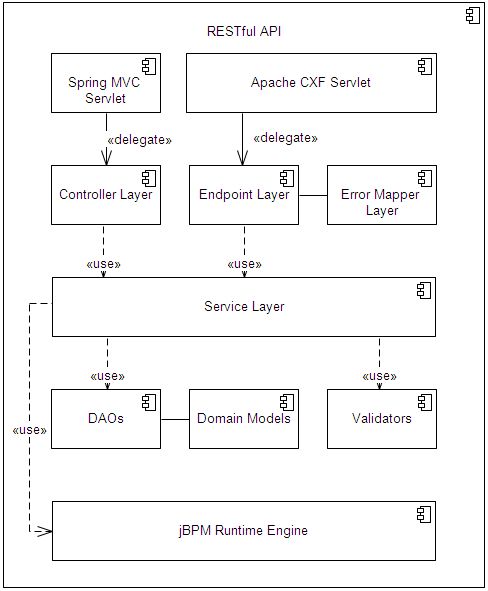
\includegraphics[width=12cm]{figures/restful_api_architecture.png}
	  	\caption{RESTful API internal architecture}
	\end{figure}
	
	Having two different servlets defined does not mean that RESTful API has duplicities. It was necessary to enable
	various capabilities and each required different approach. Both are then allowed to use the same application layers -
	Model in MVC pattern.
	
	\section{Security}\label{sec:security}
	
	RESTful API is tightly coupled with Spring ecosystem in general and heavily uses its features. Often even extends its
	implementations with custom ones. Spring framework is nicely modular and Maven enables to add only those dependencies
	that are really needed. Spring Security library is one of them.
	
	It is an authentication and access-control framework, which became standard for securing Spring-based applications.
	Enabling Spring Security for Spring application is just a matter of adding a simple filter definition to a
	\textbf{web.xml} descriptor file:
	
	\begin{lstlisting}[tabsize=2]
	<filter>
		<filter-name>springSecurityFilterChain</filter-name>
		<filter-class>
			org.springframework.web.filter.DelegatingFilterProxy
		</filter-class>
	</filter>
	<filter-mapping>
		<filter-name>springSecurityFilterChain</filter-name>
		<url-pattern>/*</url-pattern>
	</filter-mapping>
	\end{lstlisting}
	
	\subsection{Authentication}
	
	Further configuration of Spring Security is exclusively defined via Spring context configuration. In RESTful API a file
	found in META-INF/spring/\textbf{spring-security.xml}. Each CXF endpoint has a \textbf{filter chain} defined. Such
	definition example may be:
	
	\begin{lstlisting}[tabsize=2]
	<bean id="springSecurityFilterChain" 
			class="org.springframework.security.web.FilterChainProxy">
		<constructor-arg>
			<list>
				<security:filter-chain pattern="/services/user/identity"
					filters="sessionAuthenticationFilter,\
					basicAuthenticationFilter,anonymousAuthFilter,\
					exceptionTranslationFilter" />
				<security:filter-chain pattern="/services/admission"
					filters="sessionAuthenticationFilter,\
					anonymousAuthFilter,exceptionTranslationFilter" />
			</list>
		</constructor-arg>
	</bean>
	\end{lstlisting}
	
	The above shows two different filter chains that can be found in RESTful API. The first one is used in only one case -
	a UserIdentity was requested via credentials: 
	
	\begin{itemize}
		\item\label{itm:sessionAuthenticationFilter} \textbf{sessionAuthenticationFilter}

		RESTful API's custom authentication filter. It looks for \textbf{X-CTU-FIT-Admission-Session} HTTP request header,
		where a \textbf{session identifier} from \textbf{/user/identity} RESTful API's call is provided. This carries
		information about \textbf{UserIdentity}, its \textbf{Roles}, session validity, \ldots 
		\item \textbf{basicAuthenticationFilter}
		
		Default Basic HTTP Authentication implementation from Spring Security. Verifies \textbf{username} and
		\textbf{password} against Faculty's \gls{LDAP} for employees or RESTful API's database for imported
		\textbf{Admissions}. During the import, \textbf{UserIdentity} is created for each \textbf{Admission}.
		\item\label{itm:anonymousAuthFilter} \textbf{anonymousAuthFilter}
		
		A fallback filter, which sets \textbf{Anonymous Identity} into Security Context, when no \textbf{Identity} has been
		set by previous members of the filter chain.
		\item\label{itm:exceptionTranslationFilter} \textbf{exceptionTranslationFilter}
		
		Translates an Exception thrown during security filter chain processing into HTTP response if possible. 
	\end{itemize}
	
	The later one is a standard security filter chain used for every other use case in RESTful API:
	
	\begin{itemize}
		\item \textbf{sessionAuthenticationFilter}
		\item \textbf{anonymousAuthFilter}
		\item \textbf{exceptionTranslationFilter}
	\end{itemize}
	
	Basically, it is missing \textbf{basicAuthenticationFilter} and therefore it requires RESTful API's session identifier
	to successfully authenticate \textbf{UserIdentity}.
	
	\subsection{Authorization}
	
	To be authenticated is not enough to use any of RESTful API's endpoints. Successful authentication prevents one from
	receiving 401 HTTP response. Each endpoint's call requires a specific \textbf{Permission}. Relationship between
	\textbf{Role} and \textbf{Permission} is M:N. Relationship between \textbf{Role} and \textbf{UserIdentity} is M:N.
	
	Without necessary \textbf{Roles}, authenticated \textbf{UserIdentity} lacks \textbf{Permissions} and such call
	will be rejected with HTTP 403 response.
	
	Endpoint's implementation methods are annotated with \textbf{@Secured} annotations, where required \textbf{Permissions}
	are specified:
	
	\lstset{language=Java}
	\begin{lstlisting}[tabsize=2]
	@Secured("PERM_WRITE_ADMISSION")
	@Consumes({ MediaType.APPLICATION_JSON,
			MediaType.APPLICATION_XML })
	@POST
	@Override
	public Response addAdmission(Admission admission) {
		validateAndDeduplicateAndStore(admission);
		return Response.created(...).build();
	}
	\end{lstlisting}
	
	The example above shows the \textbf{/admission} POST method. It is able to consume both, JSON and XML request body,
	expects \textbf{Admission} serialized object in it and requires the \textbf{PERM\_WRITE\_ADMISSION}
	\textbf{Permission}.
	
	\section{jBPM}
	
	jBPM processing machine luckily integrates with Spring quite well. In RESTful API is configured directly via Spring
	Context and its configuration is stored in \textbf{src/main/resources/META-INF/spring/jbpm.xml}.
	
	Admission business processes and its Use Cases can be simply modelled in BPMN 2.0 using a graphic tool. JBoss Community
	offers such application as Eclipse IDE plugin. All \textbf{.bpmn} processes in RESTful API have been created this way.
	
	\newpage
	\begin{figure}[h]
		\label{fig:eclipse_drools}
	  	\centering
	    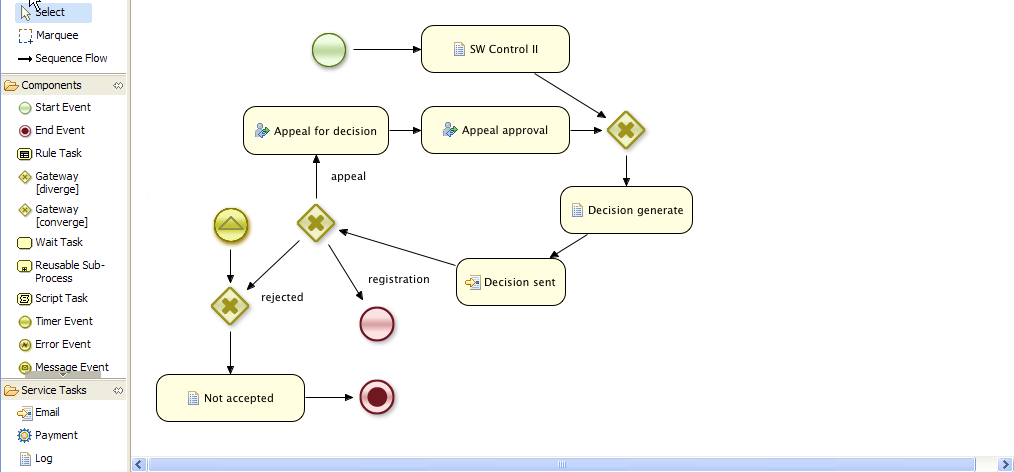
\includegraphics[width=12cm]{figures/eclipse_drools}
	  	\caption{Eclipse Drools BPMN 2.0}
	\end{figure}
	
	It is needed to differentiate between \textbf{bachelor's} and \textbf{master's} Admission processes. These are further
	split into smaller parts like registration, apology, enrollment, \ldots - also BPMN 2.0 processes. Their \textbf{.bpmn}
	representations are located in \textbf{src/main/resources/bsp} respectively \textbf{src/main/resources/msp}
	directories. Common processes are then stored in \textbf{src/main/resources/process} project directory. Their graphical
	forms can be found in Appendices section \ref{app:jbpm}.
	
	Each RESTful API call, which has some impact on Admission process should invoke appropriate task in jBPM runtime
	engine. Such action is allowed by using Spring managed \textbf{@Service} annotated implementations from
	\textbf{cz.cvut.fit.mi\_mpr\_dip.admission.jbpm} package. After RESTful API's Service and DAO layers finish their job,
	Admission is then further passed to jBPM runtime engine for evaluation. This guarantees correct state in Admission
	process.
	
	In Admission object representation, which RESTful API provides to its consumers, a state is represented by
	AdmissionState object. Modification of the state is jBPM runtime engine's responsibility. Further it handles a few
	other tasks including notification via e-mail and writing an information about changes made to the Admission object in
	logs.
	
	\section{Error handling}
	
	JAX-RS itself defines error mapping interfaces and a framework for capturing exceptional states. Apache CXF, used as
	implementation of JAX-RS in RESTful API, handles several common errors such as authentication, authorization and bad
	request body format. Returns appropriate response, when error mapper is registered. CXF servlet has to be configured to
	do so:
	
	\lstset{language=XML}
	\begin{lstlisting}[tabsize=2]
	<jaxrs:server id="restContainer" address="/">
		...
		<jaxrs:providers>
			...
			<ref bean="accessDeniedExceptionMapper" />
			<ref bean="businessExceptionMapper" />
			<ref bean="technicalExceptionMapper" />
			<ref bean="jaxbExceptionMapper" />
			<ref bean="webApplicationExceptionMapper" />
			<ref bean="throwableExceptionMapper" />
		</jaxrs:providers>
	</jaxrs:server>
	\end{lstlisting}
	
	All \textbf{ExceptionMapper} Spring managed beans are implementations of
	\textbf{javax.ws.rs.ext.ExceptionMapper\textless{E}\textgreater} interface, where \textbf{E} is a subclass of
	\textbf{java.lang.Throwable} being captured by this Exception Mapper.
	Besides special types of Exceptions defined by various frameworks:
	
	\begin{itemize}
		\item \textbf{AccessDeniedException}
		
		Typically produces HTTP 401 or 403 response
		\item \textbf{JaxbException}
		
		Produces HTTP 400 response
		\item \textbf{WebApplicationException}
		
		Various 4xx and in some special cases 5xx HTTP response
	\end{itemize}
	
	RESTful API defines three \uv{levels} of custom Exceptions, which are either thrown by Validation layer or some library
	used by RESTful API:
	
	\begin{itemize}
		\item \textbf{BusinessException}
		
		Exclusively thrown in Validation layer. This means an error on Client side. Request constrains are violated, Client
		is not authorized, \ldots Produces 4xx HTTP response and results in \verb|OK|\footnote{RESTful API did not produce
		any errors on server side. Client has supplied invalid request and typically by fixing problem on his side, request
		can be accepted and could result in 2xx or 3xx HTTP response.} RESTful API status.
		\item \textbf{TechnicalException}
		
		A known and recognized Exception, which is usually a wrapper for the original Exception thrown by a backend or
		database. In this case a Client cannot fix the problem on his side, but he can retry later - a cause of the problem
		is shown in the response message. Usually returns HTTP 500 response.
		\item \textbf{Throwable}
		
		An unexpected and unknown error. Most probably indicates a bug in RESTful API. Results in HTTP error 500 without
		further description as it may put some Java specific information into the message.
		
		Both TechnicalException and Throwable cause \verb|ERROR|\footnote{An error has occurred on Server side and Client
		cannot fix it by changing his request. ERROR status forces RESTful API's Logging service to be more verbose than OK
		status. It writes full Exception chain stack trace into server log with ERROR priority.} RESTful API response status.
	\end{itemize}
	
	A standardized Error Response body is used for all Exceptional states of RESTful API:
	
	\begin{lstlisting}[tabsize=2]
	<errorResponse>
		<message>Access is denied</message>
		<internalRequestId>
			33d91c25-9d42-4291-9af7-a387dbb49ffe
		</internalRequestId>
	</errorResponse>
	\end{lstlisting}
	
	From which:
	
	\begin{itemize}
		\item \textbf{message}
		
		Should tell the Client what happened, if possible.
		\item \textbf{internalRequestId} 
		
		A value generated for each RESTful API request and is its unique identifier, which is further appended to each row in
		the server log and so progress can be easily traced in it.
		Non ERROR responses contain this value in HTTP response headers.
	\end{itemize}
	
	\section{Profiling, Logging}

	An important part of business logic of each application should be its ability to inform system administrator, operation
	or even developer, what is happening and in a case of failure, why it was not able to process the task.
	
	RESTful API does not have many possibilities to choose from. Writing a system log seems to be a simple and usable
	approach.
	
	As I already mentioned, SLF4j logging API and Logback as its implementation is used. To utilize their capabilities,
	RESTful API defines and implements \textbf{LoggingService} interface. This service contains:
	
	\begin{itemize}
		\item \textbf{logRequest(BufferedRequestWrapper httpRequest)}
		
		All information from HTTP request including headers
		\item \textbf{logRequestBody(BufferedRequestWrapper httpRequest)}
		
		Copies HTTP request body InputStream and sends to Logger
		\item \textbf{logResponse(BufferedResponseWrapper httpResponse)}
		
		All information from HTTP response including headers and \textbf{status} - OK, request processing duration, HTTP
		response code
		\item \textbf{logResponseBody(BufferedResponseWrapper httpResponse)}
		
		Copies HTTP response body OutputStream and sends to Logger
		\item \textbf{logErrorResponse(BusinessException exception)}
		
		The same as \textbf{logResponse}
		\item \textbf{logErrorResponse(TechnicalException exception)}
		
		The same as \textbf{logResponse}, but the \textbf{status} is ERROR and Exception's stack trace is sent to the Logger
		\item \textbf{logErrorResponse(Throwable throwable, Integer httpResponseCode)}
		
		The same as logErrorResponse(TechnicalException exception), but \textbf{UnexpectedError} message is put into the
		response body
	\end{itemize}

	LoggingService methods are executed from \textbf{LoggingFilter}, which is an implementation of a standard
	\textbf{javax.servlet.Filter}. A single exception is executing \textbf{logErrorResponse} methods, which are invoked
	from JAX-RS Exception Mappers.
	
	To put it all together one example RESTful API successful call results in these log entries:
	
	\begin{verbatim}
	12-06-26 11:14:19.618 INFO  991a0741-d86b-4334-8134-876c5ad25967 
	admission-request 
	call-identifier=/admission/services/user/identity_GET 
	Connection=keep-alive Authorization=Basic_bGVzczpsZXNz== 
	Accept=application/xml User-Agent=Java/1.7.0_05 
	Host=localhost:9090 query=null
	12-06-26 11:14:19.633 INFO  991a0741-d86b-4334-8134-876c5ad25967 
	admission-request-body
	12-06-26 11:14:19.846 INFO  991a0741-d86b-4334-8134-876c5ad25967 
	c.c.f.m.a.a.UserIdentityAuthenticationProvider 
	Found authenticationService 
	[c.c.f.m.a.s.a.LdapAuthenticationService] for authentication 
	[LDAP]
	12-06-26 11:14:19.846 INFO  991a0741-d86b-4334-8134-876c5ad25967 
	c.c.f.m.a.a.UserIdentityAuthenticationProvider 
	Successfuly authentified [less]
	12-06-26 11:14:20.638 INFO  991a0741-d86b-4334-8134-876c5ad25967 
	admission-response 
	call-identifier=/admission/services/user/identity_GET code=200 
	duration=1024 status=OK
	12-06-26 11:14:20.638 INFO  991a0741-d86b-4334-8134-876c5ad25967 
	admission-response-body <?xml version="1.0" ...
	\end{verbatim}
	
	Each log entry contains a timestamp, \textbf{internalRequestId}, Logger name (admission-request,
	admission-request-body, \ldots) followed by information being logged, which can contain more parts separated by a
	single white space.
	
	It is a custom that application server with JEE application deployed is \uv{hidden} behind AJP or HTTP proxy, e.g.
	Apache httpd or nginx. These applications also provide some logging and profiling functionality, but to enable RESTful
	API's profiling capabilities, \textbf{duration} in ms is also sent to Logger.
	
	Logback is further configurable and allows many different log formats, outputs, log rotating etc. File log appender is
	used in production environment. Console output is configured for development.
	
	One important information is that the entire logging and file writing process is asynchronous and so it does not block
	RESTful API from completing its primary task. This is why under a high load with many concurrent users log entries
	might appear in different order than expected. However, it is very common in all enterprise production environments.

\chapter{Testing}\label{cha:testing}

	\section{Unit Testing}
	
	\cite{msdnunit}
	The primary goal of unit testing is to take the smallest piece of testable software in the application, isolate it from
	the remainder of the code, and determine whether it behaves exactly as expected. Each unit is tested separately
	before integrating them into modules to test the interfaces between modules.
	
	In other words, unit tests test class by class, method by method. If a tested class or method has a dependency, the
	dependency has to be stubbed, mocked, faked, dummied or spied. The five just named together form a set of test doubles.

	\subsection{\gls{TDD}}
	
	\cite{msdntdd}
	TDD is an advanced technique of using automated unit tests to drive the design of software
	and force decoupling of dependencies. The result of using this practice is a comprehensive suite of unit tests that can
	be run at any time to provide feedback that the software is still working. This technique is heavily emphasized by
	those using Agile development methodologies.
	
	These steps should be followed when doing TDD right:
	
	\begin{itemize}
		\item Understand the requirements of the story, work item, or feature that you are working on
		\item \textbf{Red} Create a test and make it fail
		\begin{itemize}
			\item Imagine how the new code should be called and write the test as if the code already existed.
			\item Create the new production code stub. Write just enough code so that it compiles.
			\item Run the test. It should fail. This is a calibration measure to ensure that your test is calling the correct
			code and that the code is not working by accident. This is a meaningful failure, and you expect it to fail.
		\end{itemize}
		\item \textbf{Green} Make the test pass by any means necessary
		\begin{itemize}
			\item Write the production code to make the test pass. Keep it simple.
			\item Some advocate the hard-coding of the expected return value first to verify that the test correctly detects
			success. This varies from practitioner to practitioner.
			\item If you've written the code so that the test passes as intended, you are finished. You do not have to write more
			code speculatively. The test is the objective definition of \uv{done.} The phrase \gls{YAGNI} is often used to veto
			unnecessary work. If new functionality is still needed, then another test is needed. Make this one test pass and
			continue.
			\item When the test passes, you might want to run all tests up to this point to build confidence that everything else
			is still working.
		\end{itemize}
		\item \textbf{Refactor} Change the code to remove duplication in your project and to improve the design while ensuring
		that all tests still pass
		\begin{itemize}
			\item Remove duplication caused by the addition of the new functionality.
			\item Make design changes to improve the overall solution.
			\item After each refactoring, rerun all the tests to ensure that they all still pass.
		\end{itemize}
		\item Repeat the cycle. Each cycle should be very short, and a typical hour should contain many Red/Green/Refactor
		cycles
	\end{itemize}
	
	Personally I adapted to work like this very quickly. It however has a drawback. One usually has to write 2 and more
	times more code than he would without testing. Each refactoring, that does not involve method renaming and extraction
	only, requires even more effort to update unit tests. This is why I used this approach only to test it within RESTful
	API, when developing import of admissions.
	
	Due to lack of time I continued without implementing unit tests any further. On the other hand, I encourage everyone to
	adopt this technique as it adds much more confidence and trust in developer's work.

	Frameworks that help to make unit testing a joy are e.g. JUnit and TestNG.
	
	There are several ways how to verify that production code is covered by unit tests. Very helpful tools, which are
	also available as Maven report plugins, are Cobertura, EMMA or JMockit code coverage. My personal experience is that
	this metrics should become a standard, when developing an important project. Therefore they should be set to
	100\% code coverage by unit tests, both line and branch.
	
	Another very helpful tool and Maven plugin is Findbugs. It compares the source code with a database of known best
	practices and warns the developer, if there are some places that need fixing or attention.

	\section{Integration Testing}
	
	\cite{msdnintegration}
	Integration testing is a logical extension of unit testing. In its simplest form, two units that have already been
	tested are combined into a component and the interface between them is tested. A component, in this sense, refers to an
	integrated aggregate of more than one unit. In a realistic scenario, many units are combined into components, which are
	in turn aggregated into even larger parts of the program. The idea is to test combinations of pieces and eventually
	expand the process to test your modules with those of other groups. Eventually all the modules making up a process are
	tested together. Beyond that, if the program is composed of more than one process, they should be tested in pairs
	rather than all at once.

	Integration testing identifies problems that occur when units are combined. By using a test plan that requires you to
	test each unit and ensure the viability of each before combining units, you know that any errors discovered when
	combining units are likely related to the interface between units. This method reduces the number of possibilities to a
	far simpler level of analysis.
	
	\subsection{Arquillian}
	
	It is a testing platform for the JVM that enables developers to easily create automated integration, functional and
	acceptance tests for Java middleware.
	
	Arquillian handles all the plumbing of container management, deployment and framework initialization. Moreover it
	covers all aspects of test execution, which entails:

	\begin{itemize}
		\item Managing the lifecycle of the container
		\item Bundling the test case, dependent classes and resources into a ShrinkWrap archive
		\item Deploying the archive to the container
		\item Enriching the test case by providing dependency injection and other declarative services
		\item Executing the tests inside the container
		\item Capturing the results and returning them to the test runner for reporting
		\item Integrates with familiar testing frameworks (e.g., JUnit, TestNG), allowing tests to be launched using existing
		IDE, Ant and Maven test plugins
	\end{itemize}
	
	RESTful API uses integration tests from two sources:
	
	\begin{itemize}
		\item Spring Roo generated for JPA Entities
		
		Each domain model is tested via Spring Roo unit and integration tests.
		\item handcrafted via Arquillian
		
		Again, due to lack of time, I just wanted to test it by myself and to demonstrate, how such tests should look like.
		This is why only a few integration tests can be found in RESTful API. They do not cover all endpoint and cover only
		positive flow.
	\end{itemize} 

	\section{Regression Testing}

	\section{Performance Testing}
\chapter{Conclusion}\label{cha:conclusion}
\chapter{Conclusion}\label{cha:conclusion}

\bibliography{mybibliographyfile}

\appendix

\printglossaries

\chapter{Build and Deploy}\label{app:deploy}



\end{document}
